\documentclass[full.tex]{subfiles}


\graphicspath{ {assets/note3/} }


\providecommand{\notenum}{3}


\begin{document}
    \thispagestyle{firstpage}
    \vspace*{2\baselineskip}
    \section*{Wallets and Cryptography}
    
    The average Bitcoin user often first downloads a \textbf{wallet} to manage funds. Analogous to storing dollars in a physical wallet for convenience, wallet software holds Bitcoin or any other cryptocurrency for users, depending on the wallet. This note is dedicated to various uses of Bitcoin wallets and how wallet cryptography keeps everyone safe.
    
    \section*{Bitcoin vs Gmail Address Creation}
    
    To review public and private keys in Bitcoin, let's compare them with Gmail accounts. When generating a Bitcoin public/private key pair, the user comes up with a private key which generates a corresponding public key via ECDSA as mentioned in the previous note. The set of possible private keys is so large that it is cryptographically safe to just generate a key. (In other words, the chances of anyone guessing or using the same private key as you are very low, so don't fear.) In contrast, the average user registering for an email account with Gmail would choose an address (username) and a password. (Username and password are independent of each other in this case and are not mathematically connected as with Bitcoin.) The main difference in the generation of public and private keys in both examples is centralization. In Bitcoin, users trust the underlying security of cryptography and the negligible probability of colliding public keys. Meanwhile, Gmail users trust Google with private information and regulation of public email addresses.
    
    \section*{Base 58}
    
    Bitcoin adopts the \textbf{base 58} convention to improve the readability of addresses. Most systems use 26 uppercase letters, 26 lowercase letters, and 10 digits, totaling to 62 unique characters. To avoid confusion between visually similar characters, base 58 drops the following characters: uppercase `I,' uppercase `O,' lowercase `l,' and the digit `0,' reducing our options to 24 uppercase letters, 25 lowercase letters, and 9 digits, a total of---you guessed it---58 characters. Although visually similar characters do not fool wallet software, a few points of human failure remain, enough to warrant the use of base 58, such as reading and writing or typing out one's public key for any manual task.
    
    \section*{Bitcoin Wallets}
    
    A Bitcoin wallet's fundamental use: storing a user's private key. While some wallets allow users to transfer bitcoin as well as store a list of UTXOs, some offline wallets do not provide this functionality but are still defined as wallets. 
    
    Bitcoin wallets come in two main flavors---hot and cold---based on their relationship with the Internet. \textbf{Hot wallets} are online and connected to the Internet, as demonstrated by apps and online web-wallets. Smartphone and PC app wallets, such as Mycelium and AirBitz, store the user's private key locally. On the other hand, online services such as Coinbase and Blockchain.info store the user's private key in the cloud, giving users access their wallet from any associated device. Hot wallets excel at enhancing user experience at the risk of many security threats due to a continuous Internet connection. What happens if a computer virus infects your computer and steals the private key from your PC wallet app, or if a trusted third party managing your private information gets compromised?
    
    \textbf{Cold wallets}, on the other hand, only exist in the physical world and are never connected to the Internet, sacrificing ease of use for security. Paper wallets, hardware wallets, and brain wallets all fall under this category. Bitaddress.org is a popular website that uses the user's pseudorandom mouse movements to generate a private key, a public key, and a pair of QR codes. By either printing out or writing down the generated data, the user successfully creates a paper wallet. Hardware wallets externally sign transactions via a trusted execution environment. Users connect their hardware wallet to a PC (usually by USB) to validate unsigned and queued transactions. The hardware wallet remains offline, signs the unsigned transactions, and sends the signed transaction back to the PC to broadcast to the network. Finally, brain wallets rely on the user memorizing their own private key, typically by memorizing a series of unrelated words which hash to the private key. 
    
    \section*{Key Stretching}
    
    Regarding the aforementioned brain wallets, consider the human mind's characteristic ineptitude to generate randomness. Users attempt to maximize `randomness' between words but will never surpass a computer's efforts. We also lose some randomness by only considering words and not random characters within the base 58 character-set, exposing brain wallet to brute force attacks.
    
    Rather than abandoning brain wallets, consider \textbf{key stretching}. Hash the hidden sequence of words repeatedly rather than just once. For example, if Alice picks a sequence of words and hashes it $2^{20}$ times, making her resulting private key exponentially harder to brute force. Although private key regeneration now takes much more work, a malicious user must guess both a sequence of English words and how many times Alice's key was stretched. A small cost for a huge gain in security.
    
    \section*{Choosing a Wallet -- Multisignature Addresses}
    
    Consider a wallet owned by a company. Should one person hold the precious private key? What happens if they steal everyone else's money? Should multiple people each hold a key? \textbf{Multisignature addresses} solve this issue by requiring multiple signatures ($m$ of $n$ total signatures) to sign a transaction.
    
   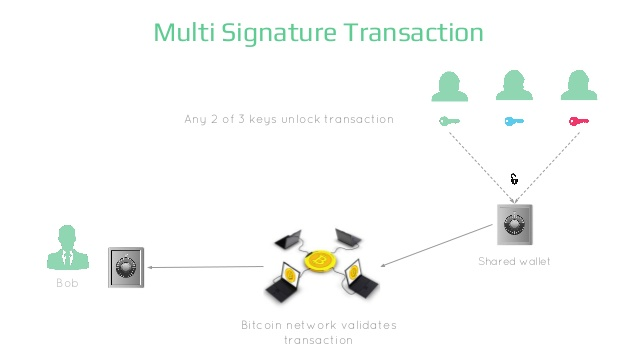
\includegraphics[scale=0.6]{multisig}

    In the image above, two of three keys of the shared wallet are necessary in order to sign a transaction. The Bitcoin network validates the transaction by checking the signature produced by the two user keys.
    
    \section*{Choosing a Wallet -- Generating New Keys}
    
    Users commonly generate new keys for every transaction to maintain privacy. As Bitcoin block explorers identify public keys associated with any given transaction, generating new keys for every transaction deters others from tracking your activity to determine how much bitcoin you own or follow your transaction history. Wallet software facilitates generation and storage of different keys by combining funds from different keys so that the user can see exactly how much bitcoin they have while enjoying reinforced security as a perk.
    
    \section*{Choosing a Wallet -- Wallet Backups}
    
    Wallet backups protect against loss, as hardware failures potentially lead to losing one's entire supply of bitcoin. However, generating new keys for every transaction poses a problem: if a user generates a new address with each transaction, then the safest backup scheme requires a new backup for every new address. This backup scheme describes \textbf{JBOK (Just a Bunch of Keys) wallets}.
    
    In \textbf{BIP (Bitcoin Improvement Proposal)} 32, the Bitcoin protocol accepted \textbf{HD (hierarchical deterministic) wallets}, where hierarchal refers to various ``ancestries" and deterministic refers to an unchanging hierarchy system, characterized by a process whereby a `child' private key comes from a `parent' private key via secure mathematical relationships, removing the burden of backing up new keys upon every transaction as with JBOK wallets. Instead, one saves a set of parent keys and later calculates child keys as needed. Each parent private key can have multiple child private keys, and each child private key can in turn be a parent private key and have children as well, defining the hierarchical property of HD wallets.  

   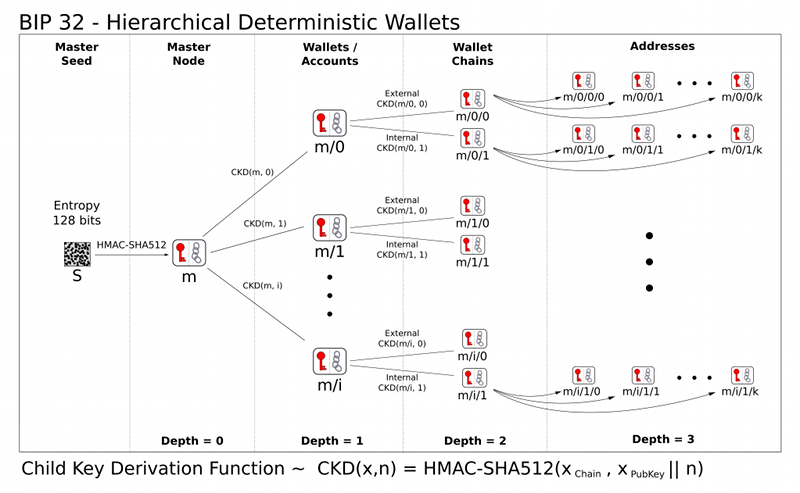
\includegraphics[scale=3.5]{bip32}
   
   Consider HD wallets in the context of complex organizations. A master seed generates and stores a secret. Financial officers or the CEO would control the master node (private key), later distributing wallets/accounts to every department of the organization, which then distributes wallets to each employee, for a manageable hierarchical structure.
   
   \section*{Choosing a Wallet -- Control \& Responsibility}
    
   We previously mentioned that Coinbase store private keys in the cloud, allowing Coinbase to spend or move funds as long as your balance stays the same whenever you use your wallet, similar to centralized bank accounts (which some Bitcoin enthusiasts do not appreciate). Centralized organizations retain your private keys, letting you use an email or phone call to retrieve your funds should you forget your Coinbase password. Otherwise, you must maintain your own backups and security.
   
   On the other hand, Mycelium and Electrum do not hold anyone's private keys. Users hold their own private keys and are responsible for their own funds. There is no recourse from these services in the case of a forgotten key or lost funds. The benefit, of course, is security since no one else controls your private keys. However, the lack of a safety net in the case of the loss of a key may scare users away.
   
   As a compromise, hardware wallets such as Case Wallet utilize a multi-signature scheme to sign a transaction. Three signatures are delegated, to the the device, Case service, and a separate backup company. When a user wants to conduct a transaction, two signatures are provided by the user's device as well as by the Case service. In the case of a lost device (i.e. a lost signature), a user can call Case and the separate backup company to get the remaining two signatures and retrieve their funds.
   
   %some sort of transition here? 
%   Nadir - probably don't need a transition since it's just the decal's format
   
   \section*{Cryptographic Hash Functions}
   
   A \textbf{cryptographic hash function}, as discussed in the previous note, maps from some \underline{arbitrarily-sized} bit string to some \underline{fixed-size} bit string. In mathematical terms: $H: \{0,1\}^{*} \mapsto \{0,1\}^{k}$
   
   The Bitcoin protocol uses the cryptographic hash function SHA-256 extensively. A cryptographic hash function only evaluates \underline{in one direction}, designed to prevent anyone from discovering a cryptographic hash function's input given an output. They are also \underline{deterministic}, meaning that the same input always yields the same output.
   
   Due to the \textbf{avalanche effect} of cryptographic hash functions, a small change in the input drastically changes the output. The avalance effect distributes outputs thoroughly. In other words, similar inputs will not produce similar outputs. Otherwise, given an output, playing a game of ``hot-or-cold" will allow malicious actors to discover the corresponding input. By putting in various inputs and comparing the output similarity, they could modify small parts of the input until the input produces the desired output. The avalance effect removes this threat.
   
   \textbf{Preimage resistance} is also a desired characteristic of good cryptographic hash functions, and describes that it should be extremely difficult to find the preimage of a cryptographic hash function output. Formally:
   \begin{align*}
       x &= \{0,1\}^{*} = \text{message (preimage)} \\
       y &= H(x) = \text{hash (output)} \\
       x &= H^{-1}(y) \rightarrow \text{finding the message should be computationally difficult}
   \end{align*}
   
   \textbf{Second preimage resistance}, also desired in a good cryptographic hash function, refers to immense difficulty in finding any value that maps to a specific input. Formally, for any given message $x$, finding any $x'$ such that $H(x') = H(x)$ should be computationally difficult.
   
   Finally, \textbf{collision resistance} in hash functions tells us that the probability of finding two inputs that map to the same output is very small. There are two equivalent ways of formalizing this statement. Suppose we have two messages $x_1$ and $x_2$;
   
   \begin{enumerate}
       \item The probability that their hashes are equal, $P\big(H(x_1) = H(x_2)\big)$, is very small, or
       \item finding \textit{any} $x_1,~x_2$ such that $H(x_1)=H(x_2)$ is computationally difficult.
   \end{enumerate}
   
   \section*{Use of Cryptographic Hash Functions}
   
   In the context of Bitcoin, we have seen cryptographic hash functions used in a number of places: miners use SHA-256 to prove the existence of relevant transactions inside of a Merkle tree; SHA-256 is used to implement Proof-of-Work; and transactions, blocks, and addresses all correspond to hash values. Outside of Bitcoin and cryptocurrencies, cryptographic hash functions find use in hash-based message authentication codes (HMACs), password verification, commitment schemes, pseudo-random number generators (PRNGs), and as the groundwork for cryptographic protocols.
   
    \section*{Simple Hash Commitment Scheme}
   
    Consider a scenario in which Alice and Bob each bet \$100 on a coin flip. Alice calls the outcome of the coin flip, and Bob flips the coin. If Alice guesses correctly, she wins \$200. Else, the money goes to Bob. In real life, this bet is easily executed. However, what if Alice and Bob are \underline{separated} and \underline{do not trust one another}? Since Alice and Bob are separated, it is very easy for Bob to cheat. Alice would send Bob her guess, and Bob would simply send back the opposite of what Alice guessed (to double his money unfairly).
    
    To solve this problem, let's use hash functions to ``bind" Alice's guess with a \textbf{commitment}:
    
    \begin{enumerate}
        \item Alice guesses the outcome of the coin flip, $B$
        \item Alice first chooses a large random number, $R$, to prevent Bob from guessing $B$ (as you will shortly see)
        \item Alice generates a commitment to the coin flip by concatenating her guess with the random number, and hashing the result: $C = H(B||R)$
        \item Alice sends this commitment to Bob
        \item Bob flips the coin and sends the result back to Alice
        \item Alice sends Bob the random number and her guess: $(R, B)$
        \item Bob then checks that $C = H(B||R)$ to verify Alice did not change her guess
        \item Both Alice and Bob can now agree on who won the \$200
    \end{enumerate}
    
    Let's examine the random number's purpose. Because of the limited options for the guess $B$, Bob could compute himself the hashes of all possible guesses. Upon receiving Alice's commitment, he would only need to compare the output to the possible hashes and work backwards to figure out Alice's guess, breaking the security. By adding the random number $R$, Bob has no way of determining which guess produced the given output so long as $H$ is a cryptographic hash function. After all, the scheme developed above depends on the effectiveness of our function $H$. Any well-designed cryptographic hash function would suffice, as illustrated by the following examples:
    
    When Bob receives the commitment $C = H(B||R)$ from Alice, if he can compute the inverse of the commitment's hash function $H^{-1}(C)$ to retrieve the input $B||R$, Bob can recover Alice's guess and play dishonestly by lying to Alice when appropriate. However, if our hash function $H$ is \underline{preimage resistant} as earlier defined, finding the input for a given output is computationally difficult, keeping both parties safe from cheating.
    
    Alice could cheat as well by sending Bob her commitment $C = H(B||R)$ as before but revealing the opposite guess $(!B,R')$ when advantageous. Alice wins the bet if she can pick $R'$ such that $C'= H(!B||R') = C$. However, if our hash function $H$ is \underline{second preimage resistant}, this scenario is deterred as well.
    
    
    

    % BEGIN KEY TERMS
    \newpage
    \thispagestyle{firstpage}
    \vspace*{2\baselineskip}
    \section*{Key Terms}
    \noindent A collection of terms mentioned in the note which may or may not have been described. Look to external sources for deeper understanding of any non-crypto/blockchain terms.
    \begin{enumerate}
        % edit within here
        \item \textbf{Avalance effect} --- In the context of hash functions: small changes to the input result in large changes to the output.
        \item \textbf{Base 58} --- Base 62 (all lowercase and uppercase letters, along with all ten digits) minus 4 particular characters to prevent mixups between similar characters.
        \item \textbf{BIP (Bitcoin Improvement Proposal)} --- Used to signal approval for a change in protocol. To gauge how much of the network supports a particular Bitcoin initiative, miners can store a piece of code in the coinbase transaction as a signal to tell the rest of the world their opinion. 
        \item \textbf{Cold wallets} --- Offline wallets, typically used for storing bitcoins long-term. By never putting the private key online, the likelihood of one's bitcoins being taken from this wallet decrease substantially.
        \item \textbf{Collision resistance} --- In the context of hash functions: the prevention of two inputs generating the same output.
        \item \textbf{Commitment} --- A hash that represents the selection of some decision while obfuscating the decision. Hashing a selection with a random number produces the commitment. With both preimage and second preimage resistance, one can commit to a particular submission or claim without revealing the claim.
        \item \textbf{Cryptographic hash function} --- See Note 1.
        \item \textbf{Hot wallets} --- Online wallets, typically holding frequently exchanged and traded bitcoins. 
        \item \textbf{Key stretching} --- Repeated hashing of a private key in the public key generation process, as opposed to only using the hash function once.
        \item \textbf{Multisignature addresses} --- Addresses associated with multiple keys, as opposed to a single private key, allowing multiple users to share an account or to produce backups. Most multisignature addresses do not only require a fraction of keys to validate a transaction, often 2-of-3 wallets.
        \item \textbf{Preimage resistance} --- A property of cryptographic hash functions. In layman's terms, it is excruciatingly difficult to create an inverse hash function that turns outputs to inputs.
        \item \textbf{Second preimage resistance} --- Another property of cryptographic hash functions. In layman's terms, it is excruciatingly difficult to find two inputs to a hash function which produce the same output.
        \item \textbf{Wallet} --- A piece of software which, at a minimum, stores one's private key. For user convenience, hot wallets also store information about past available UTXOs and protocols for creating transactions.
    \end{enumerate}
    % END KEY TERMS
\end{document}